\chapter{Plugins}
\label{cha:Plugins}

\label{sec:pluginsMenu}
\par
\index{plugin}
Les plugins sont des extensions proposant des fonctionnalit�s avanc�es, mais qui ne sont pas int�gr�es
directement dans \emph{CloudCompare} pour diff�rentes raisons. L'application peut parfaitement fonctionner sans ces fonctions, dont le domaine d'application est g�n�ralement un peu eloign� du \textit{coeur de m�tier} de \emph{CloudCompare}.\\
\par
Ils correspondent � des fichiers de type \textit{librairie dynamique} (extensions ".dll" sous Windows et ".so" sous Linux) qui sont charg�s automatiquement au d�marrage de l'application et rang�s dans le menu << Plugin >> et la barre d'outils �ponyme.\\
\par
Sont pr�sent�s ici tous les plugins \textit{officiels} de \emph{CloudCompare}. Il est toutefois possible que vous ne retrouviez pas tous ces plugins dans votre installation, ce qui encore une fois n'entrave en rien le bon fonctionnement de \emph{CloudCompare}.

%Submenu GL filters
\section{qEDL - Eye Dome Lighting}
\index{Eye-Dome Lighting}
\label{subsection:qEDL}

Plugin qEDL - \emph{Eye Dome Lighting}
\section{qSSAO - Screen Space Ambient Occlusion}
\index{qSSAO, ambient occlusion}
\label{subsection:qSSAO}

Plugin qSSAO - \emph{Screen Space Ambient Occlusion}

%Submenu Standard plugins
\section{qPCV - ShadeVis Ambient Occlusion}
\index{qPCV, ambient occlusion}
\index{Portion de Ciel Visible}
\index{eclairage@�clairage!simuler}
\label{subsection:qPCV}

\par
Cet outil permet de calculer rapidement l'illumination des points d'un nuage ou des
sommets d'un maillage par d�termination de la "\textbf{P}ortion de \textbf{C}iel \textbf{V}isible"
(P.C.V. - voir figure~\ref{fig:PCVExample}).

\begin{figure}[!htb]
\begin{center}
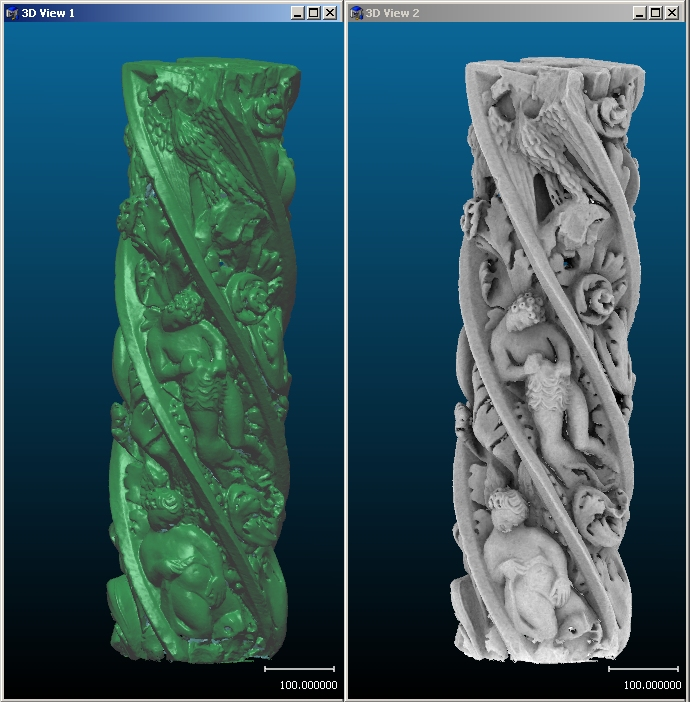
\includegraphics[width=0.6\textwidth]{Partie3_Fonctions/PCVExample.jpg}
\caption{\label{fig:PCVExample}Rendu classique avec normales (gauche) et rendu "PCV" (droite)}
\end{center}
\end{figure}

Cet �clairage consiste � calculer pour chaque point la quantit� de ciel qu'il voit, ou
autrement dit la quantit� d'�nergie lumineuse qu'il recevrait si le nuage �tait �clair�
uniform�ment. Ceci permet de colorier les points en fonction de leur profondeur
relative et fait tr�s bien ressortir le relief et la micro-g�om�trie. En pratique le calcul
est effectu� avec un algorithme �quivalent � \emph{ShadeVis} (propos� initialement par
Cignoni et al. du VCG).
\\
\par
Les deux principaux param�tres de l'algorithme, modifiables via la bo�te de dialogue associ�e
� la fonction (figure \ref{fig:PCVParamWindow}), sont :
\begin{itemize}
\item le nombre de � rayons � lumineux. Pour chaque direction d'�clairement (rayon), l'algorithme
projette, via la carte graphique, les entit�s selon cette direction et calcule la visibilit� des
points (ou des sommets d'un maillage). Cette information est accumul�e pour chaque direction et
permet de calculer l'�clairement global. Plus le nombre de rayons est grand, et plus la dynamique
est importante et les diff�rences d'�clairement entre deux points fines. Par contre, le temps de
calcul est proportionnel au nombre de rayon.
\item la r�solution du buffer de rendu. La projection des entit�s selon une direction se fait dans
un buffer vid�o dont la r�solution va jouer sur le pouvoir de s�paration entre points. Plus la
r�solution est forte, et mieux les points seront dissoci�s (d'o� un meilleur calcul de leur
�clairement propre et une meilleure finesse du r�sultat). Par contre, si la r�solution est trop
grande, outre un temps de calcul et une consommation m�moire plus importants (cela d�pend des
performances de la carte graphique), il faut aussi se m�fier du fait que le nuage peut devenir
"poreu" et laisser passer la lumi�re (voir remarque ci-dessous). Dans le cas d'un maillage ceci
ne pose pas probl�me. Les cartes graphiques actuelles assurent des performances tr�s int�ressantes
dans l'absolu, il ne faut donc pas h�siter � utiliser des valeurs importantes pour ces param�tres
(telles que les valeurs par d�faut).\\
\end{itemize}

\begin{figure}[!htb]
\begin{center}
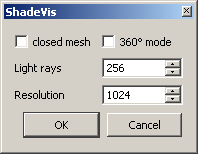
\includegraphics[width=0.3\textwidth]{Partie3_Fonctions/PCVParamWindow}
\caption{\label{fig:PCVParamWindow}Interface de param�trage de PCV}
\end{center}
\end{figure}

\par
Remarques :
\begin{itemize}
\item L'algorithme cr�e un nouveau type de champ scalaire (� PCV �) et la rampe de
couleur � Gray � (niveaux de gris) est automatiquement activ�e.
\item \textcolor[rgb]{1.0,0.0,0.0}{La lumi�re simul�e par l'algorithme PCV est consid�r�e
comme provenant de l'h�misph�re des Z positifs. Z correspondant � la direction verticale,
le nuage de points doit donc �tre orient� en cons�quence avant tout calcul.}. Si la
checkbox "360� mode" est coch�e, la lumi�re vient du globe complet et la direction ne joue plus.
\item Puisque l'illumination calcul�e par cet algorithme est un champ scalaire, il est
possible de jouer avec les potentiom�tres de saturation pour r�gler le contraste. Dans
le cas d'un maillage, on peut aussi utiliser les fonctions de moyenne et de
rehaussement du contraste (voir sections~\ref{subsection:smoothMeshSF} et
\ref{subsection:enhanceMeshSF}). Une fois les param�tres correctement r�gl�s, on peut transformer
le champ scalaire en \emph{couleurs} avec la fonction � Scalar Fields > Convert to RGB �
(section~\ref{subsection:scalarFieldConvertToRGB}).
\item L'�clairage provenant du ciel est repr�sent� de mani�re discr�te par un nombre limit� de � rayons � lumineux,
qui sont �chantillonn�s de mani�re uniforme sur l'h�misph�re (ou la sph�re compl�te
si le mode 360� est activ�). Il n'y a pas pour autant de lancer de rayons dans \emph{ShadeVis}
(on devrait plut�t parler de direction d'observation - Cf. l'article de Cignoni et al. pour
plus d'informations).
\item Dans le cas des maillages, il est possible d'acc�l�rer l'algorithme si le maillage est
ferm� (option �~closed mesh~�, activ�e par d�faut).
\item Dans le cas des nuages de points, il faut faire attention � ce que la r�solution ne
soit pas trop grande, sinon des �~trous~� peuvent appara�tre entre les points lors du
rendu interne : cceci est simplement d� au fait que la densit� d'un nuage est limit�e, et
que pour un niveau de zoom suffisant, on observera toujours des zones sans
information entre les points.
\end{itemize}

\section{qHPR - Hidden Point Removal}
\index{qHPR, filtrage de points}
\label{subsection:qHPR}

\par
La fonction \textbf{H}idden \textbf{P}oints \textbf{R}emoval tente, comme son nom
l'indique, de filtrer le nuage de points s�lectionn� de sorte � ne conserver que les
points \emph{visibles} (correspondant � la surface implicite effectivement visible depuis
le point de vue courant\index{point de vue}). Les points consid�r�s comme �tant masqu�s
sont alors cach�s. Le r�sultat d�pend donc fortement du point de vue.\\

\begin{figure}[!htb]
\begin{center}
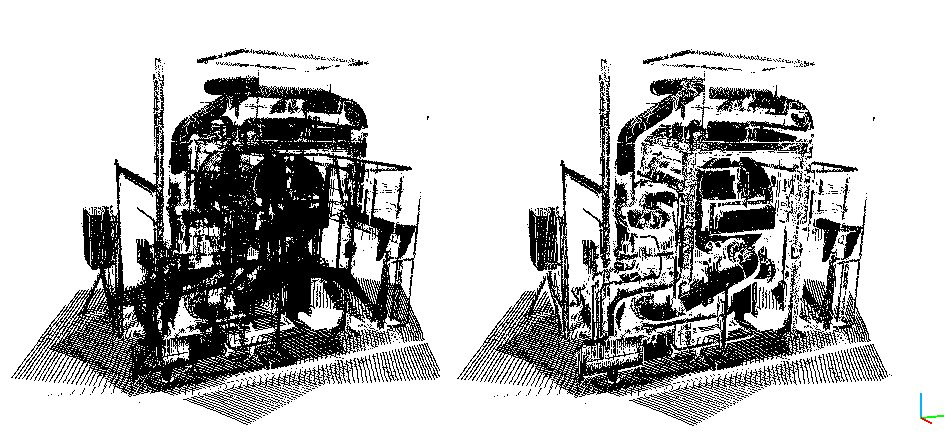
\includegraphics[width=0.5\textwidth]{Partie3_Fonctions/HPRExample.jpg}
\caption{\label{fig:PCVExample}Nuage de point complet (en haut) et nuage de point filtr� avec la technique "HPR" (en bas)}
\end{center}
\end{figure}

\par
La notion de visibilit� pour les points d'un nuage est relativement complexe � estimer.
En effet il est tr�s peu probable qu'un point soit r�ellement masqu� par
d'autres points dans un nuage, puisque cel� n�cessiterait un alignement parfait entre paires
de points ou une densit� du nuage telle que les points soient quasiment en contact. Cette fonction
approxime donc la notion de visibilit� via un calcul d'enveloppe convexe. Elle se base sur l'article
\emph{Direct Visibility of Point Sets} de Katz, Tal et Basri, SIGGRAPH 2007.
\\
\par
Pour calculer les occlusions par HPR, il est n�cessaire que le contexte graphique du nuage soit en
projection perspective (cf. section \ref{subsection:centeredPerspective}). Si ce n'est pas le cas,
un message d'erreur pr�vient l'utilisateur lui demandant d'activer la projection perspective\index{projection!pour visualisation}.
L'utilisateur doit ensuite choisir le niveau d'octree utilis� par la fonction (figure \ref{fig:HPRLevelChoice}).
Le niveau d'octree\index{octree} permet d'acc�lerer le calcul de l'enveloppe convexe (structure assez lourde)
en r�duisant le nombre de points utilis�s (par sous-�chantillonnage). Plus le niveau est �lev�, et plus
le calcul d'occlusion sera fin, mais plus le traitement sera long.
\\

\begin{figure}[!htb]
\begin{center}
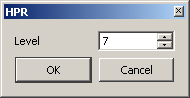
\includegraphics[width=0.3\textwidth]{Partie3_Fonctions/HPRLevelChoice}
\caption{\label{fig:HPRLevelChoice}Interface de choix de niveau d'octree}
\end{center}
\end{figure}

\par
Une fois le filtrage effectu�, celui-ci n'est valide que pour la position de cam�ra courante (et des positions tr�s
proches dans une certaine mensure). Il faut relancer l'outil pour mettre � jour le filtrage selon tout nouveau point
de vue.\\
\par
\textcolor[rgb]{1.00,0.00,0.00}{Attention, les points cach�s par cette m�thodes ne peuvent pas �tre r�-affich�s
via une m�thode ad-hoc (pour l'instant). Il faut en attendant utiliser un artifice : activer l'outil de segmentation
manuelle sur le nuage (l'ic�ne des "ciseaux" - section~\ref{subsection:graphicalSegmentation}) qui r�initialise
l'information de visibilit� par point) puis quitter ce mode.}

\section{qPCL - Point Cloud Library bridge}
\index{qPCL}
\label{subsection:qPCL}

Plugin qPCL - \emph{Point Cloud Library} bridge
\section{qPoissonRecon - Poisson Surface Reconstruction}
\index{qPoissonRecon, Poisson reconstruction}
\label{subsection:qPoissonRecon}

Plugin qPoissonRecon - \emph{surface mesh Poisson Reconstruction}
\section{qKinect - Kinect Cloud Capture}
\index{Kinect, qKinect}
\label{subsection:qKinect}

Plugin qKinect - Point cloud acquisition with a Kinect device
\section{qRansacSD - Ransac Shape Detection}
\index{qRansacSD, shape detection}
\label{subsection:qRansacSD}

Plugin qRansacSD - \emph{Ransac Shape Detection}



